\chapter{Thermal History, Decoupling, and the Primordial Soup}

Last time the cosmological problem was organized geometrically: specify a scale-factor history \(A(t)\), specify the sign of the spatial curvature, and compare the resulting model with observation. In this lecture the emphasis shifts from geometry to thermodynamics. We want the temperature history of the universe. To do that carefully, we must first say what temperature means, how radiation acquires a thermal spectrum, why that spectrum survives after equilibrium is lost, and how a few rough but powerful estimates carry us backward from the \(3\,\mathrm{K}\) microwave background to recombination, radiation domination, and the primordial electron-positron soup. These notes follow Leonard Susskind's lecture closely; selected board frames preserved by LazyingArt LLC and Video2Book are kept where they stabilize visible equations and notation.

\section{From Expansion History to Thermal History}

The lecture opens with a short recap of the strategy from the previous chapter. One begins with a cosmological model, computes its consequences, and adjusts its parameters until it agrees with the data. At this level the model is essentially specified by two ingredients,
\begin{equation}
A(t),
\qquad
k \in \{+1,0,-1\},
\end{equation}
namely the scale-factor history and the sign of the spatial curvature.

From such a model one computes, in broad outline, two kinds of observables. One is the brightness of standard sources as a function of redshift. The other is the number of visible objects as a function of redshift. At moderate redshift the first thing that matters is not so much the curvature itself as the history of the expansion. That is why one can learn a good deal about \(A(t)\) even before pinning down \(k\) with high precision. The recap is brief, and part of the transcript is garbled in this stretch, but the point is clear enough: the observational picture is consistent with a nearly flat universe and with an expansion history influenced by dark energy.

That, however, is only the hinge. What we really want to talk about now is the temperature history of the universe. The lecture narrows the focus abruptly and asks the right first question: what is temperature?

\section{What Temperature Means: Equilibrium, Scattering, and the Box Model}

Susskind insists on a strict definition. Temperature is not merely a sensation of hot and cold. Strictly speaking, temperature is a feature of thermal equilibrium. A system comes to thermal equilibrium through collisions and scattering, and it does so only if microscopic equilibration is fast compared with the timescale on which the macroscopic system changes. In cosmological shorthand we may summarize the idea as
\begin{equation}
\tau_{\mathrm{scatt}} \ll \tau_{\mathrm{exp}}.
\end{equation}
If the scattering time is much shorter than the expansion time, the system has time to settle into equilibrium.

To make that concrete, the lecture returns to the mythical box with perfectly reflecting walls. We put radiation into the box and seal it up. If there are only photons in the box, the radiation simply bounces back and forth. Photons do not efficiently scatter off one another under ordinary conditions, so a pulse of radiation does not automatically spread itself into a thermal distribution. A box of pure free radiation does not thermalize.

Now put charged particles in the box. Electrons are excellent scatterers of electromagnetic radiation. The field of the wave shakes the electron; the accelerated electron reradiates; the process is efficient. If the box contains a reasonable density of free electrons and protons, then photons, electrons, and protons exchange energy rapidly and settle into a common thermal soup.

The universe, however, is electrically neutral. In the simplest model we therefore take the contents to be photons, electrons, and protons, with equal electron and proton densities,
\begin{equation}
n_{e^-} = n_p.
\end{equation}
If the electrons and protons remain free, radiation couples strongly to them. If instead they bind into neutral hydrogen atoms, the situation changes completely. Neutral atoms scatter very weakly. In the dilute present universe they are such poor scatterers that the photons do not come to equilibrium with matter on anything like the age of the universe. That is why the present universe is not in thermal equilibrium.

There is a further point in the lecture that is easy to smooth away if one is not careful. Today the radiation and the matter are not merely weakly coupled; they are characterized by very different effective temperatures. If one assigns a temperature to the dilute matter by its kinetic energy, that temperature is not the temperature of the microwave photons. The two sectors are simply not sharing one common equilibrium state.

\subsection{Question \& Answer}

\paragraph{Question.} If the microwave background has a temperature of about \(3\,\mathrm{K}\), why can we not simply say that the universe today has temperature \(3\,\mathrm{K}\)?

\paragraph{Answer.} Because the present universe is not a single equilibrated system. The microwave photons have a blackbody spectrum that can be characterized by a temperature, but the atoms, electrons, and other forms of matter are not in equilibrium with those photons. They do not share one common temperature. The modern universe therefore does not have one global thermodynamic temperature in the strict sense in which the lecture is using the word.

\section{Blackbody Radiation, Planck's Formula, and the Thermal Wavelength}

Once the box really is in thermal equilibrium, the next question is unavoidable: what does the radiation look like? The box does not contain photons of one single wavelength. It contains a whole spectrum. We may describe the radiation by wavelength \(\lambda\) or by frequency \(\nu\), related by
\begin{equation}
\nu \lambda = c.
\end{equation}
The spectral distribution is encoded in an intensity function \(I(T,\nu)\), defined so that
\begin{equation}
dE = I(T,\nu)\, dV\, d\nu
\end{equation}
is the energy stored in a volume element \(dV\) within a frequency band \(d\nu\).

Before doing dimensional analysis, Susskind pauses over a basic but important matter of units. For his purposes temperature is essentially an energy. Boltzmann's constant \(k_B\) is only the conversion factor between customary temperature units and energy units. Thus whenever \(T\) appears in a formula, one should really think of \(k_B T\) as the energy scale.

The lecture then proceeds historically. Before quantum theory the only fundamental constant available in the theory of radiation was \(c\). If one combines \(k_B T\), \(\nu\), and \(c\), dimensional analysis drives one to a Rayleigh--Jeans type law. Because the lecture openly wobbles over powers of \(c\) and the precise convention for \(I\), the safe and faithful statement is the proportional one:
\begin{equation}
I_\nu^{\mathrm{classical}} \propto k_B T\, \nu^2.
\end{equation}
This law has the correct low-frequency behavior. But as a complete law it is a disaster. It keeps growing with \(\nu\), so the total energy in the box would diverge. That is the ultraviolet catastrophe.

The cure is to introduce a new constant, Planck's constant \(h\), and with it the blackbody formula:
\begin{equation}
I_\nu \propto \frac{h\nu^3}{e^{h\nu/(k_B T)}-1}.
\end{equation}
Again, the lecture uses this formula for its shape and scaling, not for its exact convention-dependent normalization. The crucial point is that the denominator contains the dimensionless ratio \(h\nu/(k_B T)\).

At low frequency we set
\[
x=\frac{h\nu}{k_B T},
\qquad
x\ll 1,
\]
and expand \(e^x-1 \approx x\). Then
\begin{align}
I_\nu
&\propto
\frac{h\nu^3}{e^{h\nu/(k_B T)}-1}
\approx
\frac{h\nu^3}{h\nu/(k_B T)}
=
k_B T\, \nu^2.
\end{align}
So the Planck spectrum reproduces the classical result for small \(\nu\). The real change comes when \(h\nu/(k_B T)\) is no longer small.

\begin{figure}[t]
\centering

\includegraphics[width=0.78\textwidth]{lecture_07_figure_02.png}
\caption{Thermal-wavelength inequality on the board. The upper line is clipped, but the crossover condition is evident. The faint lower-board remnants are not sharp enough to carry independent mathematical weight.}
\end{figure}

The board evidence is especially useful here. The upper line is partially cut off, but its meaning is clear enough:
\begin{equation}
\frac{h\nu}{kT}\gtrsim 1.
\end{equation}
The lower line rewrites the same threshold in wavelength language:
\begin{equation}
\frac{hc}{kT}\gtrsim \lambda.
\end{equation}
The lecture repeatedly treats this not as a precision formula but as the crossover scale separating the classical region from the quantum-suppressed region. In the cleaned notation used in these notes we summarize it as
\begin{equation}
E = h\nu,
\qquad
\lambda_{\mathrm{th}} \sim \frac{hc}{k_B T}.
\end{equation}
The relation \(E=h\nu\), written explicitly during the units discussion, is what makes the exponential argument dimensionless: both \(h\nu\) and \(k_B T\) are energies.

There is another important simplification that the lecture lingers on. Ignoring overall constants that only change normalization, one may write schematically
\begin{equation}
I(\nu,T) \propto T^3\, f\!\left(\frac{\nu}{T}\right).
\end{equation}
Thus the shape of the blackbody curve depends only on the ratio \(\nu/T\). Changing the temperature mainly rescales the curve along the frequency axis. That fact will become essential once the box begins to expand.

\begin{figure}[t]
\centering
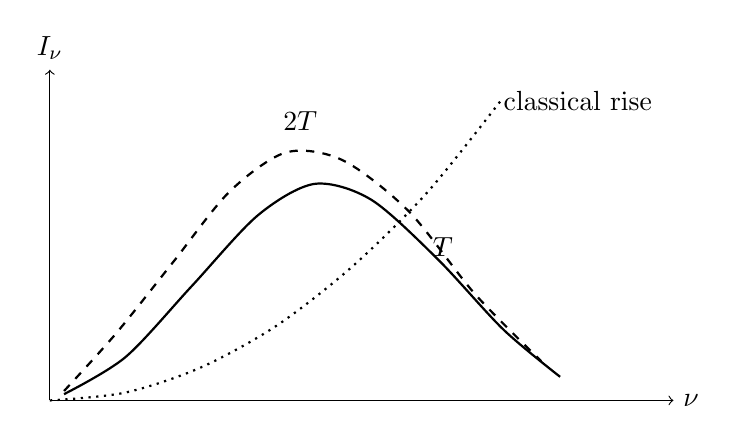
\begin{tikzpicture}[x=1.2cm,y=1.0cm]
\draw[->] (0,0) -- (6.6,0) node[right] {$\nu$};
\draw[->] (0,0) -- (0,4.2) node[above] {$I_\nu$};

\draw[dotted,thick] plot[smooth] coordinates
{(0.0,0.0) (0.8,0.10) (1.6,0.42) (2.4,0.95) (3.2,1.70) (4.0,2.65) (4.8,3.85)};

\draw[thick] plot[smooth] coordinates
{(0.15,0.08) (0.8,0.55) (1.5,1.45) (2.2,2.35) (2.8,2.75) (3.4,2.55) (4.1,1.80) (4.8,0.90) (5.4,0.30)};

\draw[dashed,thick] plot[smooth] coordinates
{(0.15,0.12) (0.7,0.85) (1.3,1.75) (1.9,2.65) (2.5,3.15) (3.1,3.05) (3.8,2.40) (4.5,1.35) (5.2,0.50)};

\draw (2.65,3.30) node[above] {$2T$};
\draw (3.95,1.95) node[right] {$T$};
\draw (4.70,3.80) node[right] {classical rise};
\end{tikzpicture}
\caption{Schematic blackbody spectra. The dotted curve indicates the classical continuation responsible for the ultraviolet catastrophe. The solid and dashed curves show the quantum turnover and the approximate rescaling of the spectrum with temperature.}
\end{figure}

The lecture then makes a rough but suggestive observational point. Most of the photons in the present universe lie near a wavelength of about a millimeter. Using the thermal-wavelength correspondence, one would associate that with a temperature of about \(3\,\mathrm{K}\). At first this is only a rough translation between wavelength and temperature; by itself it does not prove equilibrium. Later, however, one measures the full spectrum and finds that the microwave background really does fit a blackbody curve to extremely high precision.

\subsection{Question \& Answer}

\paragraph{Question.} Why is the classical formula such a disaster, and what does the new constant \(h\) actually buy us?

\paragraph{Answer.} The classical formula keeps increasing with frequency, so it predicts an infinite total energy in the box. With only \(c\) available, there is no way to build a function that turns the curve over. The introduction of \(h\) creates the dimensionless ratio \(h\nu/(k_B T)\). That ratio is small at low frequency, where the classical law is recovered, but it becomes large at high frequency, where the exponential suppression cuts off the spectrum. In the logic of the lecture, \(h\) is the new scale that makes a finite blackbody spectrum possible.

\paragraph{Question.} Did Planck arrive at this formula from the same electron-proton box model used here?

\paragraph{Answer.} No. The lecture is careful on this point. Planck did not begin with the modern plasma picture. He used empirical curve fitting together with what was already known from Wien's displacement law, and in that way identified a new constant \(h\). The deeper derivation from general principles came later. Here we are using the box model pedagogically, not historically.

\section{Expansion, Decoupling, and the Frozen Blackbody Spectrum}

We now return from the box to the universe. Imagine that the box begins at sufficiently high temperature that electrons and protons are ionized. Then the charged particles scatter radiation efficiently, the whole system is in equilibrium, and the photon spectrum is blackbody.

Now expand the box. As it expands, the contents do work and cool. Eventually the temperature falls low enough that electrons and protons combine into atoms. This is recombination. At that point the effective scatterers disappear, the radiation ceases to couple strongly to matter, and the photons decouple. The lecture is explicit that decoupling is the right word for the radiation, while recombination describes the formation of neutral atoms.

One might think that once equilibrium is lost, the blackbody form should disappear. But the lecture's central observation is exactly the opposite. The blackbody shape is frozen in. The reason is simple and beautiful. Expansion stretches every photon wavelength by the same factor. If the linear size of the box grows by a factor \(\alpha\), then the radiation undergoes the update
\begin{equation}
\lambda \mapsto \alpha \lambda,
\qquad
T \mapsto \frac{T}{\alpha}.
\end{equation}
Since the shape of the spectrum depends only on \(\nu/T\), stretching every wavelength uniformly is equivalent, for the radiation, to lowering the temperature. In cosmological form,
\begin{equation}
\lambda \propto A,
\qquad
T \propto A^{-1}.
\end{equation}

This is why the microwave background today still has the blackbody form. It is not because present radiation and present matter are still in equilibrium. The lecture stresses exactly the contrary. The spectrum is blackbody today because it acquired that form at an earlier ionized epoch and then preserved that form as the universe expanded.

There is also a useful change of emphasis here. The \(3\,\mathrm{K}\) temperature of the microwave background is not the statement that the universe now is a \(3\,\mathrm{K}\) plasma. It is the statement that the radiation today is the expanded remnant of a once-thermal spectrum.

\subsection{Question \& Answer}

\paragraph{Question.} How can a blackbody spectrum remain blackbody after equilibrium has already been lost?

\paragraph{Answer.} Because after decoupling the relevant operation is a uniform stretching of all wavelengths, not continued equilibration. Once the radiation has the blackbody shape, multiplying every wavelength by the same factor simply relabels the same shape by a lower temperature. That is exactly what expansion does to freely propagating radiation.

\section{Recombination Temperature from the Boltzmann Tail}

Having established that the microwave background is a thermal relic, the lecture turns to an estimate. At what temperature did recombination, and therefore decoupling, occur?

The naive answer is the obvious one. Hydrogen ionizes at about
\begin{equation}
\epsilon_{\mathrm{ion}} \approx 13.6\,\mathrm{eV},
\end{equation}
so perhaps one should say that ionization persists until the characteristic photon energy is of order \(13.6\,\mathrm{eV}\), namely
\begin{equation}
k_B T \sim \epsilon_{\mathrm{ion}}.
\end{equation}
This is the simple first guess, and the lecture introduces it explicitly before overturning it.

\begin{figure}[t]
\centering

\includegraphics[width=0.72\textwidth]{lecture_07_figure_03.png}
\caption{Photon-energy notation and the photon-to-electron ratio on the board. The visible exponential is incomplete in the frame, but the transcript makes clear that the intended factor is the Boltzmann weight \(e^{-\epsilon/(kT)}\).}
\end{figure}

The correction comes from abundance. There are vastly more background photons than electrons or protons:
\begin{equation}
\frac{N_\gamma}{N_e} \sim 10^8.
\end{equation}
This is an observational fact extracted from the matter inventory of the universe together with the blackbody photon density of the CMB. Therefore the right question is not whether the average photon is ionizing. The right question is whether the high-energy tail contains enough photons above threshold.

Susskind introduces the notation \(\epsilon\) for photon energy and uses the Boltzmann distribution
\begin{equation}
P(\epsilon) \propto e^{-\epsilon/(k_B T)}.
\end{equation}
Strictly speaking the board frame only shows the beginning of this expression, but the transcript completes it unambiguously. If we evaluate the tail at the ionization energy and multiply by the number of photons available per electron, the criterion for roughly one ionizing photon per atom is
\begin{equation}
10^8 e^{-\epsilon_{\mathrm{ion}}/(k_B T)} \sim 1.
\end{equation}
This is the lecture's crucial step. Taking logarithms gives
\begin{align}
\frac{\epsilon_{\mathrm{ion}}}{k_B T}
&\sim \ln 10^8
\approx 20,
\\[4pt]
k_B T
&\sim
\frac{\epsilon_{\mathrm{ion}}}{20}.
\end{align}
So the recombination temperature is not of order the full ionization energy. It is lower by a factor of order \(20\). Later in the lecture Susskind entertains the possibility that a more careful treatment pushes the factor closer to \(40\), and he emphasizes that the estimate is only meant to be rough. But the physics is already in view: because there are so many photons, the tail matters far more than the average.

The lecture then carries this into a temperature estimate. Using the rough factor \(20\), and taking the point only at the level of order of magnitude, one arrives at
\begin{equation}
T_{\mathrm{dec}} \sim 4\times 10^3\,\mathrm{K}.
\end{equation}
The exact number is not the lesson. The lesson is that recombination happens far below the naive ionization temperature.

A further lecture beat is worth preserving here. The photon-to-electron ratio being used is taken to be the ratio for the microwave background photons, not for all photons of all origins. Starlight is irrelevant to this early epoch, both because it was not yet present and because even today it makes up only a tiny fraction of the photon population.

\subsection{Question \& Answer}

\paragraph{Question.} Why does recombination happen at a temperature much lower than the hydrogen ionization energy?

\paragraph{Answer.} Because the average photon is not the correct standard. There are about \(10^8\) photons per electron. Even when the typical photon energy is far below \(13.6\,\mathrm{eV}\), the exponentially small tail of the distribution still contains enough photons above threshold to keep hydrogen ionized. Recombination waits until the tail itself becomes too sparse.

\subsection{Question \& Answer}

\paragraph{Question.} If recombination emits \(13.6\,\mathrm{eV}\) photons, why does that not leave a dramatic line in the final microwave background?

\paragraph{Answer.} Because as long as the process unfolds slowly enough, the radiation remains very close to thermal equilibrium while recombination is occurring. Emission, absorption, and scattering keep reprocessing the photons so that the spectrum stays near the equilibrium curve. Only if freeze-out were too abrupt would one expect a pronounced bump to survive.

There is one more point from the same part of the lecture. The ratio \(N_\gamma/N_e \sim 10^8\) is treated as essentially frozen in all the way back to decoupling, because between decoupling and much hotter epochs there is no important mechanism for changing the total number of CMB photons or the total number of electrons and protons.

\section{Scale Factor, Last Scattering, and the Limit of Electromagnetic Observation}

Now the recombination estimate becomes geometrical. The characteristic wavelength of the radiation we see today is the expanded remnant of the characteristic wavelength at decoupling, so
\begin{equation}
\frac{\lambda_0}{\lambda_{\mathrm{dec}}}
=
\frac{A_0}{A_{\mathrm{dec}}}
=
\frac{T_{\mathrm{dec}}}{T_0}.
\end{equation}
Here \(T_0\) means the temperature of the microwave background itself, not the temperature in this room and not the kinetic temperature of the dilute matter in space.

With
\[
T_0 \approx 3\,\mathrm{K},
\qquad
T_{\mathrm{dec}} \sim 4\times 10^3\,\mathrm{K},
\]
we obtain
\begin{equation}
\frac{A_0}{A_{\mathrm{dec}}}
\sim
\frac{4\times 10^3\,\mathrm{K}}{3\,\mathrm{K}}
\sim 10^3.
\end{equation}
So the universe has expanded by about a factor of one thousand since decoupling.

This is the first clean landmark in the backward thermal history. Before decoupling the universe was ionized and therefore optically opaque. Light scattered strongly from the charged plasma and did not travel freely across cosmological distances. After decoupling the universe became transparent and the radiation we now call the CMB began its essentially free propagation.

The lecture then switches from algebra to geometry. Looking farther away in space means looking farther back in time. Electromagnetic astronomy therefore presents the universe to us in shells: nearby shells correspond to recent times, more distant shells correspond to earlier times, and the outermost shell accessible to ordinary light is the surface of last scattering. Telescopes that measure the CMB are effectively looking back to that surface.

The lecture also returns, near the end, to a common confusion. The CMB is older than the galaxies. But the fact that we see the CMB back to decoupling tells us nothing directly about whether there are galaxies today beyond the region from which their light can reach us. It only tells us how far electromagnetic radiation carries direct information backward. What supports the usual extrapolation is the observed homogeneity of galaxies out to the greatest distances we can survey: there is no sign of a sharp edge.

\subsection{Question \& Answer}

\paragraph{Question.} Does decoupling mark the end of all possible observation, or only the end of ordinary electromagnetic observation?

\paragraph{Answer.} Only the latter. The lecture's point is that electromagnetic radiation cannot show us epochs earlier than decoupling, because the pre-decoupling universe was opaque to light. But much more weakly interacting messengers, such as neutrinos, could in principle emerge from earlier epochs. Gravitational radiation would be less impeded still. Thus decoupling is the observational wall for light, not necessarily for every conceivable messenger.

\section{Earlier Landmarks: Equality, Pair Creation, and the Asymmetry Puzzle}

Having reached decoupling, the lecture keeps going backward. The next landmark is matter-radiation equality. Matter and radiation scale differently with the expansion:
\begin{equation}
\rho_m \propto A^{-3},
\qquad
\rho_r \propto A^{-4}.
\end{equation}
Therefore
\begin{equation}
\frac{\rho_m}{\rho_r} \propto A.
\end{equation}
As we go backward and \(A\) gets smaller, radiation becomes more important.

Susskind estimates the present ratio by a deliberately crude counting argument. There are about \(10^8\) CMB photons per proton. Each photon carries characteristic energy of order \(10^{-4}\,\mathrm{eV}\). A proton carries about \(10^9\,\mathrm{eV}\). Thus, if we first ignore dark matter,
\begin{equation}
\left(\frac{\rho_m}{\rho_r}\right)_0
\sim
\frac{10^9\,\mathrm{eV}}{10^8 \times 10^{-4}\,\mathrm{eV}}
\sim 10^5.
\end{equation}
Then the lecture interrupts itself and corrects the estimate: dark matter was forgotten. Including it raises the matter density by about a factor of ten, so
\begin{equation}
\left(\frac{\rho_m}{\rho_r}\right)_0 \sim 10^6.
\end{equation}
Since \(\rho_m/\rho_r \propto A\), equality occurred when the scale factor was smaller than today by the same factor:
\begin{equation}
\frac{A_{\mathrm{eq}}}{A_0} \sim 10^{-6},
\qquad
\frac{T_{\mathrm{eq}}}{T_0} \sim 10^6.
\end{equation}
Thus going backward beyond decoupling, one reaches an earlier epoch in which radiation, not matter, controlled the energy budget and therefore the expansion law.

\subsection{Question \& Answer}

\paragraph{Question.} Why does the lecture keep emphasizing ratios of \(A\) rather than absolute values of \(A\)?

\paragraph{Answer.} Because in a nearly flat universe the absolute normalization of the scale factor is not directly meaningful. A flat space does not possess a finite radius of curvature whose value \(A\) could literally measure. What is physically meaningful is the expansion factor between two epochs. Thus \(A_0/A_{\mathrm{dec}}\), \(A_0/A_{\mathrm{eq}}\), and similar ratios carry content, while an isolated value of \(A\) does not.

The lecture then pushes to still higher temperature. When the temperature reaches about
\begin{equation}
T \sim 10^{10}\,\mathrm{K},
\qquad
\frac{A_0}{A} \sim 10^{14},
\end{equation}
the characteristic photon energy is of order
\begin{equation}
\epsilon_\gamma \sim 1\,\mathrm{MeV}.
\end{equation}
The threshold discussion is intentionally qualitative here: the lecture treats the relevant scale as being of order the electron rest mass. Once photons have energies of that order, pair creation becomes possible:
\begin{equation}
\gamma\gamma \leftrightarrow e^- e^+.
\end{equation}
Now the number of electrons and positrons is no longer determined by what survives to the present. It is determined by equilibrium at the current temperature. This is what Susskind means by saying that their abundance is no longer determined by ``memory of the future.''

In that hot plasma the electrons, positrons, and photons are all present in roughly comparable abundance, up to a tiny excess. The sum \(N_{e^-}+N_{e^+}\) changes because pair creation and annihilation change it continuously. But the difference does not change:
\begin{equation}
N_{e^-}-N_{e^+}=\mathrm{constant}.
\end{equation}
In the intermediate regime emphasized in the lecture, before proton-antiproton pair creation becomes important, this conserved excess is essentially the proton number required by neutrality.

The lecture then makes its final turn. If the total number of electrons plus positrons in the hot soup is of the same order as the photon number, while the surviving excess is only of order the present electron number, then
\begin{equation}
\frac{N_{e^-}-N_{e^+}}{N_{e^-}+N_{e^+}} \sim 10^{-8}.
\end{equation}
So in the primordial electron-positron soup there was roughly one excess electron for every \(10^8\) electron-positron pairs.

This turns the old puzzle upside down. One might have asked: why are there so many photons? The lecture answers: that is not the sharp question. The sharp question is why the excess of matter over antimatter is so tiny.

\subsection{Question \& Answer}

\paragraph{Question.} Why is the real mystery the tiny excess \(N_{e^-}-N_{e^+}\), and not simply the large number of photons?

\paragraph{Answer.} Because once the temperature is high enough for pair creation, photons, electrons, and positrons are all present in comparable abundance. If there had been exact equality between electrons and positrons, cooling would eventually have annihilated essentially all of them away. What survives is precisely the imbalance. Thus the weird number is not that there were many photons in the soup, but that there was only one excess electron per \(10^8\) pairs.

The lecture then sharpens the question once more. If the world at very high temperature were symmetric between particles and antiparticles, one would naturally expect equal numbers of electrons and positrons. Why then is the difference nonzero at all? And if it is nonzero, why is it so small? This is exactly where the lecture stops. The microscopic explanation of that asymmetry is deferred to the next session.

There is one more observational remark at the end. Across the visible universe the sign of the excess appears to be the same. We do not see antigalaxies sending us antinuclei. The lecture regards such large-scale sign coherence as far too big to be a local statistical fluctuation. At the same time it insists on restraint: beyond the horizon we do not directly know what there is.

\section{Summary}

The lecture begins with geometry and turns to thermodynamics. Temperature is defined through equilibrium, equilibrium through scattering, and the box model teaches us immediately why free charges matter and neutral atoms do not. Once the box is in equilibrium, radiation is described by a blackbody spectrum, and the key dimensionless ratio \(h\nu/(k_B T)\) tells us where the classical description fails and quantum suppression takes over.

From there the lecture becomes cosmological. Expansion stretches wavelengths, so a blackbody spectrum can survive long after matter and radiation fall out of equilibrium. The present CMB is therefore understood as a frozen thermal relic. Using the huge ratio \(N_\gamma/N_e \sim 10^8\) together with the Boltzmann tail, one finds that recombination occurs not at the full ionization temperature of hydrogen but at a much lower temperature, of order \(4\times 10^3\,\mathrm{K}\). That estimate then becomes the statement that the universe has expanded by about a factor of \(10^3\) since decoupling.

Going backward still farther, one reaches matter-radiation equality and then the electron-positron pair-production era, where equilibrium fixes particle abundances directly. The lecture ends not with a closed theory, but with a sharpened problem: the primordial soup was almost symmetric, with only one excess electron for roughly every \(10^8\) electron-positron pairs. That tiny excess, not the mere abundance of photons, is the real puzzle carried forward to the next lecture.